\documentclass[journal]{IEEEtran}

\usepackage{amsmath,amssymb}
\usepackage{array}
\usepackage{booktabs}
\usepackage{cite}
\usepackage{graphicx}
\usepackage{multirow}
\usepackage{tabularx}
\usepackage{url}

\newcommand{\ours}{FedTwin-CryptID}
\newcommand{\phitwin}{\boldsymbol{\phi}}
\newcommand{\thetavec}{\boldsymbol{\theta}}
\newcommand{\risk}{\rho}

\begin{document}

\title{\ours: Federated Fixed-Evidence Calibration and Audit for Multimedia Copy Review}

\author{Chandrasen~Pandey}

\maketitle

\begin{abstract}
Collaborative multimedia copy review often depends on evidence held by different platforms, rights holders, archives, and regional monitoring clients. Centralizing raw media, embeddings, labels, or infringement records can expose copyrighted content, private moderation decisions, business-sensitive evidence, and user metadata. This paper presents \ours, a privacy-aware fixed-evidence calibration and audit layer above existing visual-copy, audio-fingerprint, descriptor, or retrieval pipelines. It calibrates compact query-reference evidence across nonidentically distributed clients without exporting raw media or raw embeddings; it does not introduce a new retrieval representation, copy localizer, audio fingerprint, or ownership-adjudication mechanism. The default detector is a standardized logistic head over precomputed scores, reliability-weighted terms, and cross-modal products, with client and category fields excluded to limit contextual leakage. Experiments compare centralized and local training with federated averaging, proximal federation, simulated secure aggregation, a quantized transport proxy, real 2048-bit Paillier aggregation, and client personalization. On a checksum-verified, asset-disjoint public video-copy label tier, plain and protected federated heads obtain 0.9186 area under the precision--recall curve after rounding. The evaluation also reports receiver-operating-characteristic area, false-positive rate at 95\% recall, calibration error, review workload, query-level ranking, poisoning stress, receipt tampering, and cryptographic overhead. Separate visual-descriptor and audio tiers test modality-specific evidence without claiming synchronized audiovisual fusion. The results support human-review triage and signed audit logging, not automated enforcement, formal privacy, or superiority over end-to-end copy-localization systems.
\end{abstract}

\begin{IEEEkeywords}
Multimedia copy review, video copy retrieval, audio fingerprinting, federated learning, secure aggregation simulation, Paillier aggregation, fixed-evidence calibration, content provenance, auditability, privacy-aware machine learning.
\end{IEEEkeywords}

\section{Introduction}

Video copy detection, near-duplicate retrieval, audio fingerprinting, and multimedia provenance have matured into important research areas. TMM and multimedia-retrieval work studies robust video-copy matching, partial-copy localization, near-duplicate retrieval, compact hashing, temporal/spatial verification, fine-grained video similarity, and recent self-supervised regional-token localization \cite{wu2009realtime,douze2010image,chou2015pattern,song2013multiple,hao2017smvh,kordopatis2019fivr,feng2022vcsl,shao2021transvcl,lu2024selfsupervised,liu2013survey_ndvr}. Large-scale indexing and learned visual representations further shape modern copy-review pipelines \cite{rui2019survey,gosselin2021deep,johnson2019billion,radford2021clip,arnab2021vivit}. Audio fingerprints provide complementary robustness for copied soundtracks, remixes, previews, short clips, and time-scale modifications \cite{wang2003shazam,cano2005review,baluja2008waveprint,carletti2019audio,defferrard2017fma,gemmeke2017audioset}. Practical copy review, however, is increasingly collaborative: streaming platforms, social networks, rights owners, archives, and regional monitoring entities each observe only part of the infringement surface. A detector that requires all parties to upload raw media or embeddings is often operationally and legally unattractive.

The question addressed here is therefore not whether video or audio copies can be detected in a centralized benchmark. It is whether a fixed-evidence multimedia calibration and audit layer can be trained across non-IID clients without pooling raw media, raw embeddings, or full evidence records. Federated learning trains models across distributed clients \cite{mcmahan2017fedavg,kairouz2021advances,yang2019federated,li2020fedprox,karimireddy2020scaffold,reddi2021fedopt,li2021ditto}, but multimedia copy review has additional constraints: hard negatives are visually or acoustically similar to true copies; transformations may affect only one modality; client distributions are non-IID; evidence receipts must be auditable; and protected update accounting must not destroy utility. Secure aggregation \cite{bonawitz2017secureagg} and homomorphic encryption \cite{paillier1999public,cheon2017ckks,acar2018surveyhe,pham2020flhe,wang2019privacy} motivate update-protection mechanisms. Content-provenance systems and evidence ledgers can anchor commitments \cite{bui2020archangel,collomosse2019content,c2pa2026spec,weng2016multiparty,shafiq2022blockchain}, but they should not be overclaimed as piracy prevention.

This paper proposes \ours, a raw-media non-export federated pair-evidence calibration and audit system for multimedia copy review. The word ``twin'' is used only in a bounded data-model sense: the system maintains a structured, media-free state for each query-reference candidate pair, not a full content simulator, retrieval index, or copy-localization model. Each pair state records modality evidence, reliability, transformation descriptors, model digest, and evidence-receipt commitments. Client and category context are treated as optional audit/sensitivity fields, not as default detector inputs.

The contributions are fourfold. First, we define a media-free fixed-evidence calibration formulation with an explicit invariant feature policy and leakage notes for optional context fields. Second, we evaluate a federated compact-head and audit layer under centralized, local, FedAvg, FedProx, SecureAgg simulation, a quantized transport proxy, real Paillier compact-update summation, personalized FL, and FedOpt-style baselines. Third, we add signed, salted, media-free receipt chains that record commitments and model digests without storing raw media or embeddings. Fourth, we report multi-tier detection, calibration, query-ranking, leakage, poisoning, dropout, receipt, Paillier, and rare-prevalence analyses that expose both useful operating regions and failure modes.

The remainder of this paper is organized as follows. Section II reviews related work in multimedia copy detection, federated learning, protected aggregation, and provenance auditing. Section III formulates the fixed-evidence copy-review task and threat model. Section IV presents the FedTwin-CryptID framework. Section V describes the datasets, benchmark tiers, baselines, and metrics. Section VI reports detection, ablation, open-set, robustness, privacy, and audit results. Section VII discusses deployment scope, while Section VIII covers reproducibility, ethics, and limitations. Section IX concludes the paper.

\begin{table*}[!t]
\centering
\caption{Claim-to-evidence map and explicit boundaries.}
\label{tab:claim-evidence}
\scriptsize
\begin{tabularx}{\textwidth}{p{0.25\textwidth} p{0.36\textwidth} X}
\toprule
Claim & Evidence in this paper & Boundary \\
\midrule
Fixed-evidence calibration can be trained across distributed clients without exporting raw media or raw embeddings. & VCSL public-label, VCSL ISC visual-descriptor, and FMA audio tiers with centralized, local, FedAvg, FedProx, SecureAgg-simulation, quantized-proxy, personalized, and FedOpt-style variants. & The head consumes precomputed pair evidence; it is not a new visual representation, audio fingerprint, or segment-localization network. \\
Protected-update accounting preserves compact-head utility in the evaluated setting. & SecureAgg simulation and a quantized transport proxy match plain FedAvg within numerical tolerance; Paillier encrypts compact update sums. & No production SecureAgg deployment, threshold key management, differential privacy, collusion proof, or ciphertext-domain media scoring is claimed. \\
Media-free receipt chaining supports audit traceability. & Signed receipt-chain verification and tamper checks succeed for generated logs with salted commitments, model digests, public keys, signatures, and previous-link hashes. & A receipt proves commitment consistency and ordering under a signing key; it does not prove correctness, ownership, or legal infringement. \\
Query-level ranking exposes deployment risk. & VCSL public-label Recall@K, mAP, fixed-review-budget precision, and 1:1-1:10000 candidate-pool analyses. & These are public label/topology candidate metrics, not full segment-overlap localization metrics over raw video descriptors. \\
\bottomrule
\end{tabularx}
\end{table*}

\section{Related Work}

Visual copy detection and near-duplicate retrieval provide the closest multimedia foundation. Classical TMM systems combine visual signatures, local matching, temporal verification, and scalable retrieval \cite{wu2009realtime,douze2010image,chou2015pattern,song2013multiple,hao2017smvh}. FIVR and ViSiL pushed fine-grained incident retrieval and spatio-temporal similarity learning toward realistic partial-copy and event-level settings \cite{kordopatis2019fivr,kordopatis2019visil}. VCSL and VCDB emphasize segment-level copy localization and partial-copy evaluation \cite{feng2022vcsl,jiang2015vcdb}. These methods are strong upstream evidence providers, but they usually assume centralized access to features, labels, or indexes.

Audio fingerprinting is complementary because copied soundtracks can survive visual edits or appear in short clips \cite{wang2003shazam,cano2005review,baluja2008waveprint}. Watermarking and tamper analysis are related but different: they either embed marks or detect manipulation artifacts, while this work calibrates copy-pair evidence and records commitments without claiming forensic authenticity \cite{cayre2005watermarking,cox2007watermarking,sitara2018digital}. Federated, secure, and personalized learning methods motivate the cross-client training layer \cite{mcmahan2017fedavg,kairouz2021advances,li2020fedprox,karimireddy2020scaffold,reddi2021fedopt,li2021ditto}. Secure aggregation and homomorphic encryption protect aggregate updates in different threat models \cite{bonawitz2017secureagg,paillier1999public,cheon2017ckks,acar2018surveyhe}. Provenance systems such as ARCHANGEL and C2PA motivate auditable records, but in \ours{} the ledger only records salted commitments, not media, embeddings, or legal conclusions \cite{bui2020archangel,c2pa2026spec}.

\begin{table*}[!t]
\centering
\caption{Positioning against representative multimedia, FL, and provenance work.}
\label{tab:positioning}
\scriptsize
\begin{tabularx}{\textwidth}{p{0.18\textwidth} p{0.16\textwidth} p{0.16\textwidth} X}
\toprule
Work family & Strength & Not covered & Role in \ours{} \\
\midrule
TMM copy retrieval \cite{wu2009realtime,douze2010image,chou2015pattern} & Visual matching and scalable near-duplicate retrieval & Cross-client protected training and media-free receipts & Supplies the upstream visual-copy evidence that the calibration head consumes. \\
FIVR/ViSiL/VCSL/VCDB \cite{kordopatis2019fivr,kordopatis2019visil,feng2022vcsl,jiang2015vcdb} & Fine-grained/segment-level video copy evaluation & Raw-media non-export collaborative calibration & Used as benchmark lineage; not replaced by the proposed layer. \\
Audio fingerprints \cite{wang2003shazam,cano2005review,baluja2008waveprint} & Robust audio identification and short-clip evidence & Visual fusion and federated audit & Supplies the audio branch evidence for soundtrack and clip-copy scenarios. \\
Watermarking/forensics \cite{cayre2005watermarking,cox2007watermarking,sitara2018digital} & Embedded or passive evidence & Collaborative score calibration & Complementary; no watermark or authenticity proof is required. \\
FL/personalization \cite{mcmahan2017fedavg,li2020fedprox,reddi2021fedopt,li2021ditto} & Cross-client optimization under non-IID data & Multimedia copy-pair evidence and audit receipts & Provides training mechanisms for the compact calibration head. \\
Secure/HE aggregation \cite{bonawitz2017secureagg,paillier1999public,cheon2017ckks} & Protected update aggregation & Full encrypted multimedia inference & Protects compact updates; Paillier is evaluated only for additive update sums. \\
Provenance ledgers \cite{bui2020archangel,c2pa2026spec,weng2016multiparty} & Commitment and provenance records & Detector training or legal ownership proof & Anchors signed media-free receipt commitments after review decisions. \\
\bottomrule
\end{tabularx}
\end{table*}

\section{Problem Formulation and Threat Model}

Let $q$ be a query media item and $r$ a candidate reference. The detector receives a compact pair state
\begin{equation}
\phitwin(q,r)=[s_v,s_a,s_t,m,\eta_v,\eta_a,g,z],
\end{equation}
where $s_v$ is visual-copy similarity, $s_a$ is audio-copy similarity, $s_t$ is temporal consistency, $m$ captures modality agreement, $\eta_v$ and $\eta_a$ are reliability indicators, $g$ denotes transformation or scenario context, and $z$ denotes permitted non-media metadata. The default detector excludes direct client/category identifiers. The label $y\in\{0,1\}$ indicates whether the pair is a copy or non-copy. The compact head estimates
\begin{equation}
 p_{\thetavec}(y=1\mid q,r)=\sigma(f_{\thetavec}(\phitwin(q,r))),
\end{equation}
where $\sigma$ is the logistic function. Heavy visual and audio feature extraction are frozen in the first implementation; the evaluated layer is the collaborative fusion/calibration head exchanged across clients.

There are $K$ clients. Client $k$ owns $\mathcal{D}_k=\{(\phitwin_i,y_i)\}_{i=1}^{n_k}$ and the federated objective is
\begin{equation}
\min_{\thetavec}\sum_{k=1}^{K}\frac{n_k}{n}\mathcal{L}_k(\thetavec),\quad
\mathcal{L}_k=\frac{1}{n_k}\sum_{i\in\mathcal{D}_k}\ell(f_{\thetavec}(\phitwin_i),y_i).
\end{equation}
At round $t$, FedProx replaces the local objective by
\begin{equation}
\mathcal{L}^{\mathrm{prox}}_k(\thetavec;\thetavec_t)=\mathcal{L}_k(\thetavec)+\frac{\mu}{2}\lVert\thetavec-\thetavec_t\rVert_2^2,
\end{equation}
with $\mu=0.02$ in the reported runs. FedAvg uses the data-weighted mean of local updates; personalization starts from that global head and fine-tunes only on the client's local calibration rows.
Non-IID behavior arises from content category, transformation family, visual-copy family, or client-specific label surfaces.

The threat model includes honest-but-curious aggregation infrastructure, clients that do not want to reveal raw media or raw embeddings, and auditors who need to verify detection records after the fact. The server may observe aggregate updates and receipt hashes, but not raw media. The current work does not claim malicious-client robustness proof, differential privacy, full encrypted inference, DRM enforcement, or legal ownership adjudication. These boundaries are important because the system is intended as copy-review triage and audit support.

\section{System Design}

\begin{figure*}[!t]
  \centering
  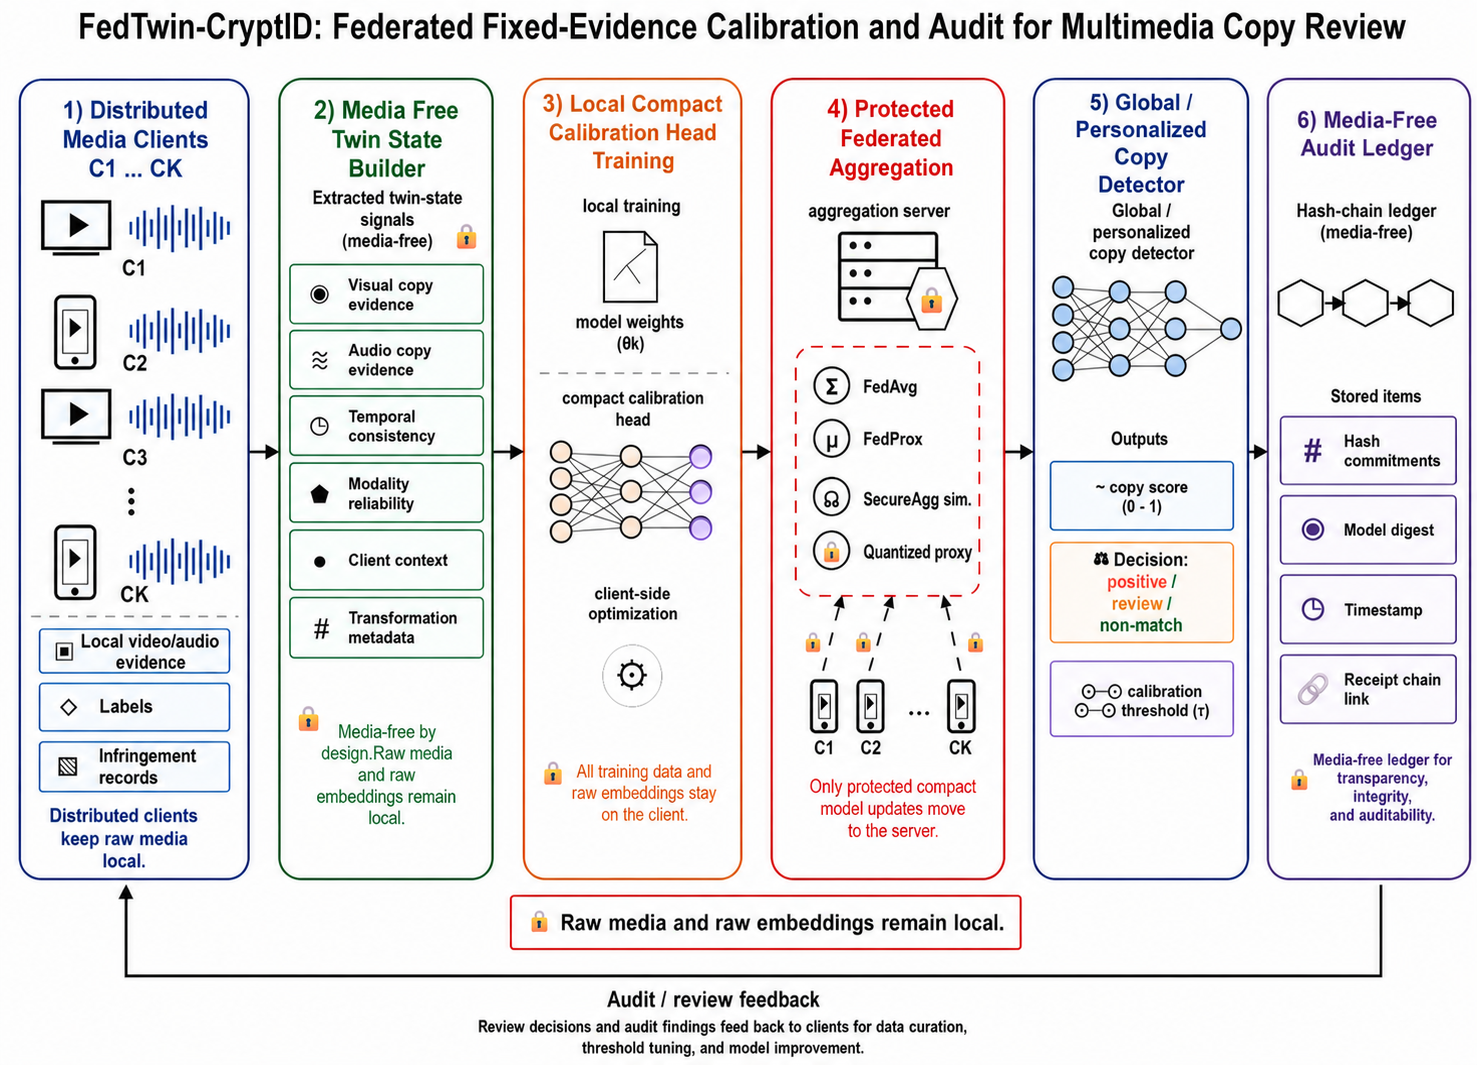
\includegraphics[width=0.78\textwidth]{figures/Figure1_FedTwin_CryptID_Framework_tmm.png}
  \caption{Overall \ours{} framework. Each client keeps raw multimedia assets and raw embeddings local, constructs media-free pair-evidence features, trains a compact local calibration head, and sends only protected model updates for aggregation. During online detection, the global or personalized detector produces copy scores and review flags; only salted commitments, signatures, model digests, and receipt-chain links are anchored for audit.}
  \label{fig:framework}
\end{figure*}

\begin{figure*}[!t]
  \centering
  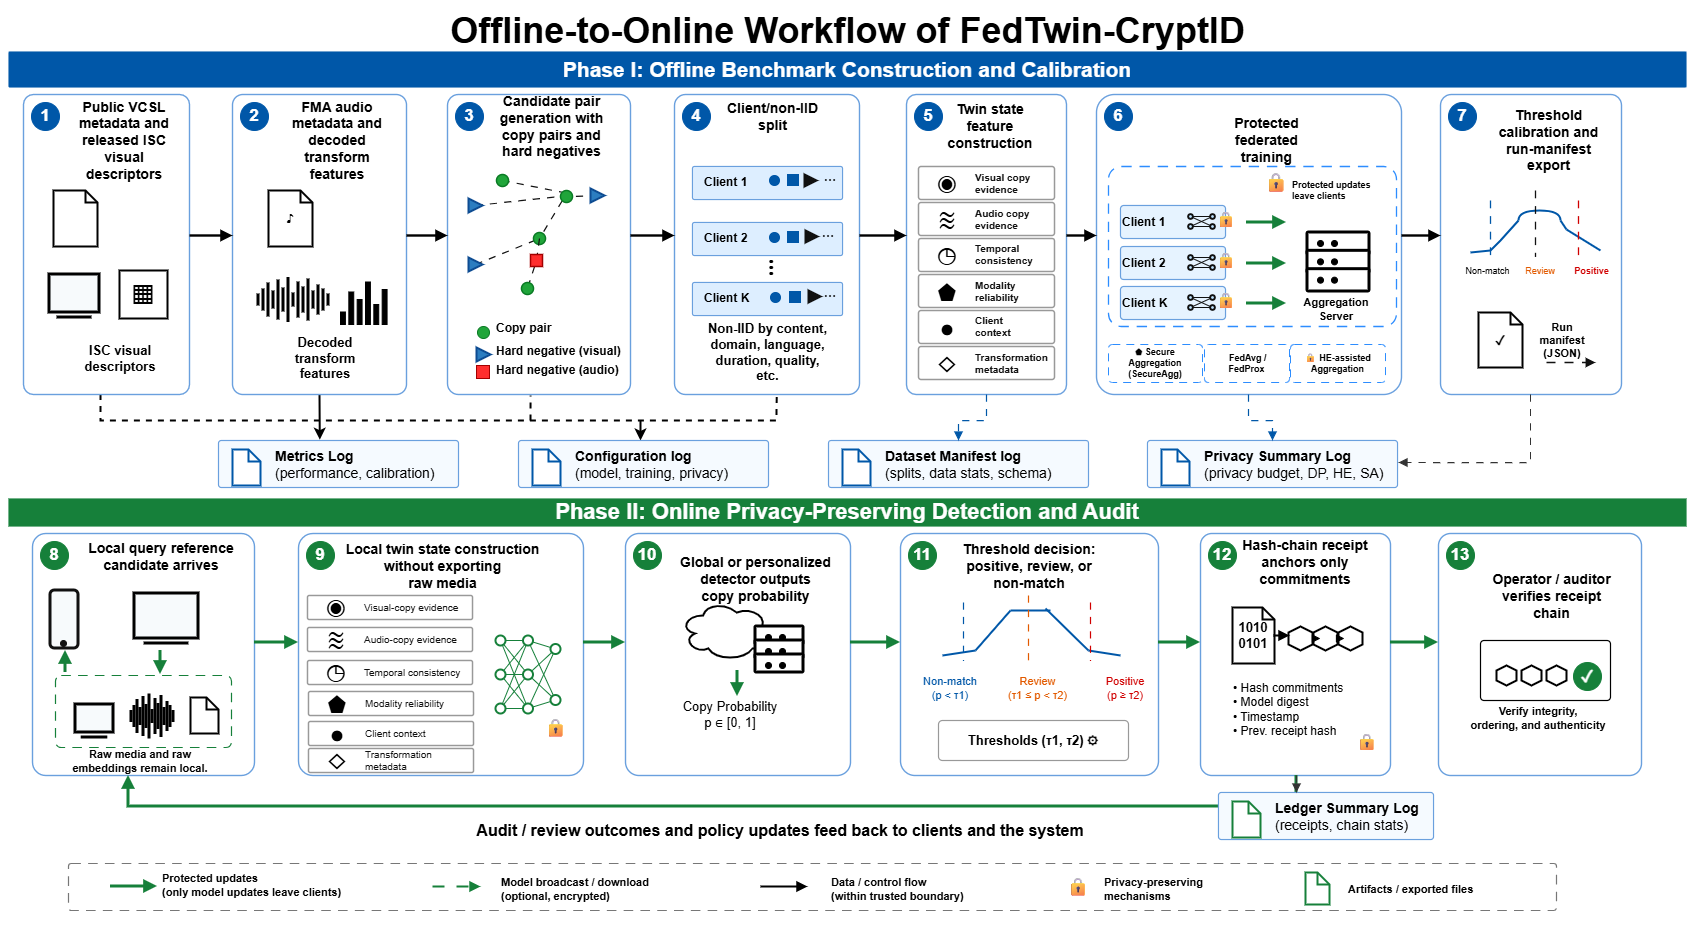
\includegraphics[width=0.88\textwidth]{figures/Figure2_FedTwin_CryptID_Workflow.drawio.png}
  \caption{Offline-to-online workflow of \ours. Offline construction builds public visual/audio benchmark pairs, client splits, transformations, and calibration artifacts. Online detection constructs local pair-evidence states, runs protected federated calibration, and anchors only media-free evidence receipts.}
  \label{fig:workflow}
\end{figure*}

Fig.~\ref{fig:framework} separates three concerns that are often mixed in piracy-detection systems: multimedia copy evidence, protected collaborative learning, and auditable evidence recording. In the offline stage, each client constructs pair labels, transformation manifests, and fixed evidence vectors from local or public benchmark resources. In each communication round, clients train the compact head for a few local epochs and transmit an update. Plain FedAvg is the reference; the SecureAgg simulation implements deterministic pairwise masks and dropout-cancellation checks but is not a production protocol; the quantized transport proxy measures numeric error and byte expansion but is not encryption; the Paillier microbenchmark performs real additive encrypted summation for compact quantized updates. FedProx, FedAdam, FedYogi, and personalized fine-tuning are included because non-IID client behavior is visible in visual tiers.

For each positive or review decision, the client can issue a receipt
\begin{equation}
 R=H(q)\Vert H(r)\Vert H(\thetavec)\Vert H(\phitwin)\Vert t\Vert H(R_{\mathrm{prev}}),
\end{equation}
where $H(\cdot)$ is a hash, $t$ is a timestamp or monotone counter, and the ledger anchors $H(R)$ together with a signature. The receipt proves commitment consistency and chain order under the signing key. It does not prove that a detection is correct, that a claimant owns the content, or that legal infringement occurred.

\begin{table*}[!t]
\centering
\caption{Implementation details for the compact fixed-evidence head. Client/category fields are used only in sensitivity audits and are excluded from the default detector.}
\label{tab:implementation}
\scriptsize
\begin{tabularx}{\textwidth}{p{0.20\textwidth} p{0.23\textwidth} p{0.16\textwidth} X}
\toprule
Component & Setting & Dimension/status & Notes \\
\midrule
Score roots & video, audio, temporal, max-modality, mean-modality & 5 roots & Used by score-only logistic baseline. \\
Default invariant roots & video, audio, reliability-weighted video, reliability-weighted audio, modality product & 5 roots & Designed to avoid direct context while retaining interpretable agreement terms. \\
Polynomial map & squares and pairwise products & 20-D selected map & Standardized on train split and applied to test split. \\
All-field audit map & all feature families after expansion & 151-D & Used only to measure whether context improves accuracy or leaks identity. \\
Optional context & category, genre, client/domain indicators & excluded by default & Leakage audit recovers client/category when these fields are included. \\
Fusion head & logistic regression with bias & compact head & Heavy visual/audio encoders are frozen upstream. \\
Optimization & 30-40 FL rounds, 5-8 local epochs, L2=$10^{-4}$ & FedAvg/FedProx/FedOpt & FedProx uses $\mu=0.02$; FedAdam/FedYogi use $\beta_1=0.9$, $\beta_2=0.99$. \\
Protection & plain, SecureAgg simulation, quantized proxy, Paillier & measured per run & Only Paillier is encrypted; simulation/proxy modes are not production cryptography. \\
Audit record & signed salted hash chain & media-free receipt & Stores commitments, model digest, feature digest, signature, and previous-link hash. \\
\bottomrule
\end{tabularx}
\end{table*}

\begin{table}[!t]
\centering
\caption{Compact training and audit protocol used in the experiments.}
\label{tab:protocol}
\scriptsize
\begin{tabularx}{\columnwidth}{p{0.18\columnwidth} X}
\toprule
Stage & Operation \\
\midrule
Pair state & Build fixed media-free evidence from local visual/audio candidates. \\
Local fit & Train a standardized compact calibrator for $E$ local epochs. \\
Protection & Send plain, masked-simulation, quantized-proxy, or Paillier compact update. \\
Aggregation & Average updates; FedProx/FedOpt/personalization handle non-IID effects. \\
Decision & Score candidate pairs and flag positives or review-required pairs. \\
Receipt & Sign salted commitments to media hashes, model digest, feature digest, and previous receipt. \\
\bottomrule
\end{tabularx}
\end{table}

\section{Experimental Protocol}

\begin{table*}[!t]
\centering
\caption{Executable benchmark tiers. Rows and client counts are generated from pulled manifests.}
\label{tab:benchmark-tiers}
\scriptsize
\begin{tabularx}{\textwidth}{p{0.16\textwidth} p{0.16\textwidth} p{0.09\textwidth} r r r X}
\toprule
Tier & Source & Modality & Clients & Train rows & Test rows & Purpose \\
\midrule
Synthetic twin$^{\dagger}$ & Generated pair features & A+V & 20 & 15,000 & 5,000 & Pipeline, FL, privacy, and ledger sanity validation. \\
VCSL public labels & Public VCSL metadata and labels & V/meta & 11 & 5,000 & 1,800 & Asset-disjoint public label-topology tier with within-split hard negatives. \\
VCSL ISC visual$^{\dagger}$ & Released ISC frame descriptors & V & 11 & 6,000 & 3,000 & Real visual-descriptor tier using variable-length 256-D frame descriptors. \\
FMA audio 20 s$^{\dagger}$ & FMA-small MP3 and metadata & A & 8 & 12,000 & 6,000 & Real-audio transformed-copy and same-genre hard-negative tier. \\
FMA audio 5 s$^{\dagger}$ & FMA-small short clips & A & 8 & 12,000 & 6,000 & Short-clip stress tier for partial audio evidence. \\
\bottomrule
\end{tabularx}
\end{table*}

Table~\ref{tab:benchmark-tiers} summarizes the evaluation. The synthetic tier is a system-validation tier and is not presented as the main scientific evidence. VCSL public labels evaluate label-topology copy evidence and hard negatives; the regenerated audit assigns complete positive connected components to frozen train/test partitions, samples negatives only within a partition, rejects duplicate directional pairs in the canonical constructor, and verifies zero asset-identity overlap. Rows marked $\dagger$ are checksum-incomplete archived experiments and are retained as exploratory context, not confirmatory evidence. Released VCSL ISC descriptors and FMA audio provide separate visual and audio evidence; they do not establish synchronized audiovisual performance. Runs use seeds 31, 37, and 41. The comparison includes random scoring, single-modality similarity, centralized heads, local-only training, FedAvg, FedProx, SecureAgg-simulation FedAvg, quantized-proxy FedAvg, Paillier update summation, FedAdam/FedYogi, and personalized FedAvg. We report PR-AUC, ROC-AUC, FPR at 95\% recall, Brier score, 15-bin expected calibration error, Recall@$K$, mAP, recall at fixed review budgets, and expected human-review workload. Confidence intervals cluster resamples by query; paired permutation and bootstrap comparisons use the same held-out examples and Holm correction across method comparisons. Exact client, pair, positive, negative, and query counts are released with each result row.

\section{Results}

\subsection{Multitier Detection}

\begin{figure*}[!t]
  \centering
  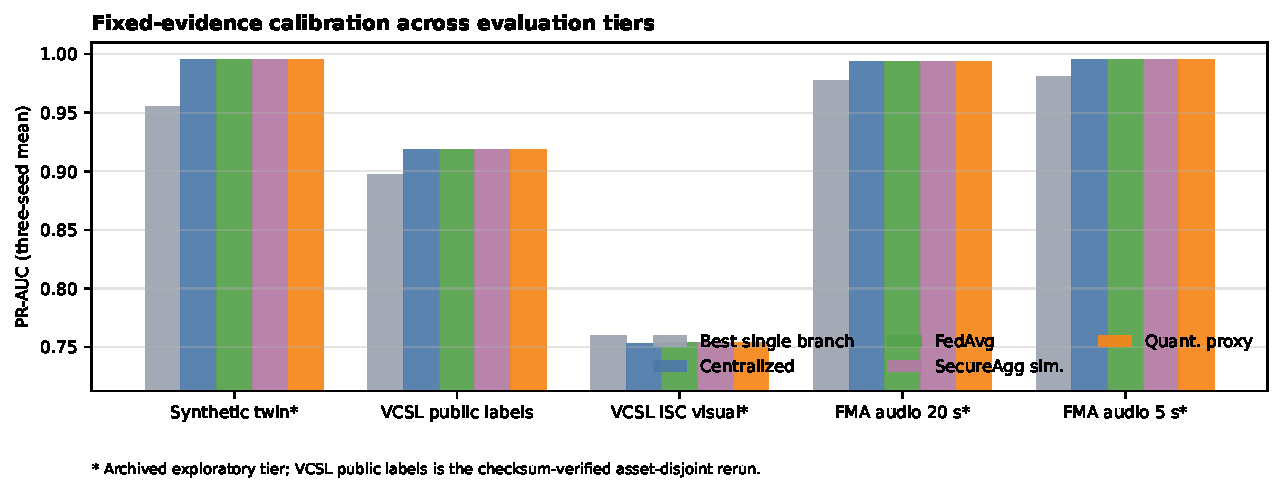
\includegraphics[width=0.90\textwidth]{figures/fig01_multitier_pr_auc.pdf}
  \caption{Multitier PR-AUC across synthetic, visual, and real-audio benchmark tiers. Protected modes distinguish SecureAgg simulation, quantized transport accounting, and real Paillier compact-update summation.}
  \label{fig:multitier-pr-auc}
\end{figure*}

\begin{table*}[!t]
\centering
\caption{Fixed-evidence calibration results. Values are mean PR-AUC over seeds; the final column reports the best overall mean and standard deviation. $\dagger$ denotes checksum-incomplete archived results retained as exploratory context.}
\label{tab:main-results}
\scriptsize
\begin{tabularx}{\textwidth}{p{0.15\textwidth} p{0.17\textwidth} r r r r r r}
\toprule
Tier & Best single branch & Centralized & FedAvg & SecureAgg sim. & Quant. proxy & Best protected FL & Best overall \\
\midrule
Synthetic twin$^{\dagger}$ & 0.9552 & \underline{0.9956} & \textbf{0.9957} & \textbf{0.9957} & \textbf{0.9957} & \textbf{0.9957} & \textbf{0.9957}$\pm$0.0005 \\
VCSL public labels & 0.8974 & 0.9183 & 0.9186 & 0.9186 & 0.9186 & \underline{0.9186} & \textbf{0.9186}$\pm$0.0254 \\
VCSL ISC visual$^{\dagger}$ & \underline{0.7596} & 0.7527 & 0.7538 & 0.7538 & 0.7538 & \underline{0.7596} & \textbf{0.7760}$\pm$0.0090 \\
FMA audio 20 s$^{\dagger}$ & 0.9773 & 0.9936 & 0.9935 & 0.9935 & 0.9935 & \underline{0.9939} & \textbf{0.9940}$\pm$0.0008 \\
FMA audio 5 s$^{\dagger}$ & 0.9808 & 0.9949 & 0.9950 & 0.9950 & 0.9950 & \textbf{0.9953} & \textbf{0.9953}$\pm$0.0010 \\
\bottomrule
\end{tabularx}
\end{table*}

The asset-disjoint VCSL public-label row is the confirmatory result. Centralized multimodal calibration obtains 0.9183 PR-AUC; plain FedAvg, SecureAgg simulation, and the quantized transport proxy each obtain 0.9186 after rounding, and FedProx is also 0.9186. Thus the compact protected modes preserve the corresponding plain-head utility, but do not establish a material accuracy gain. The descriptor and audio rows in Fig.~\ref{fig:multitier-pr-auc} and Table~\ref{tab:main-results} are archived exploratory evidence: VCSL ISC previously favored local calibration, while FMA favored calibrated and personalized heads. Because the archived raw-input hashes are unavailable, these rows are not used for confirmatory claims.

\begin{figure*}[!t]
  \centering
  \begin{minipage}{0.32\textwidth}
    \centering
    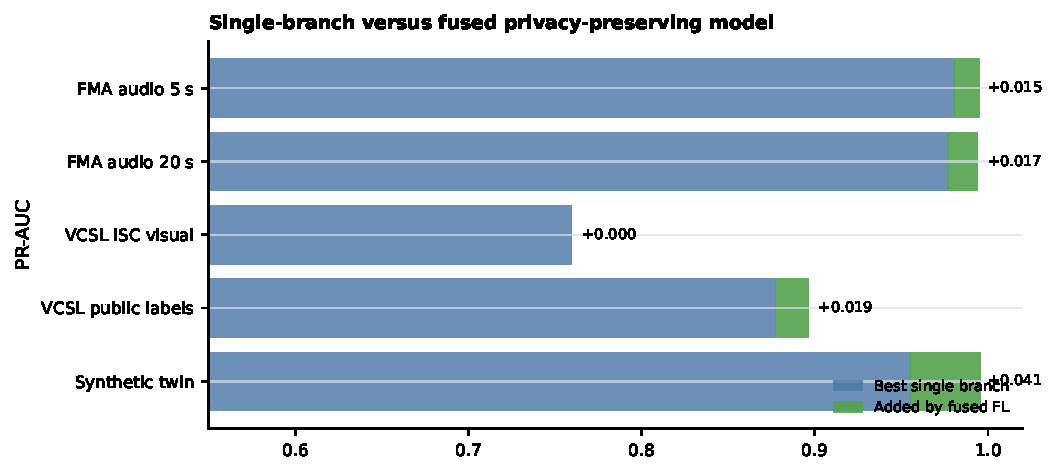
\includegraphics[width=\linewidth]{figures/fig02_single_vs_fused_gain.pdf}
  \end{minipage}\hfill
  \begin{minipage}{0.32\textwidth}
    \centering
    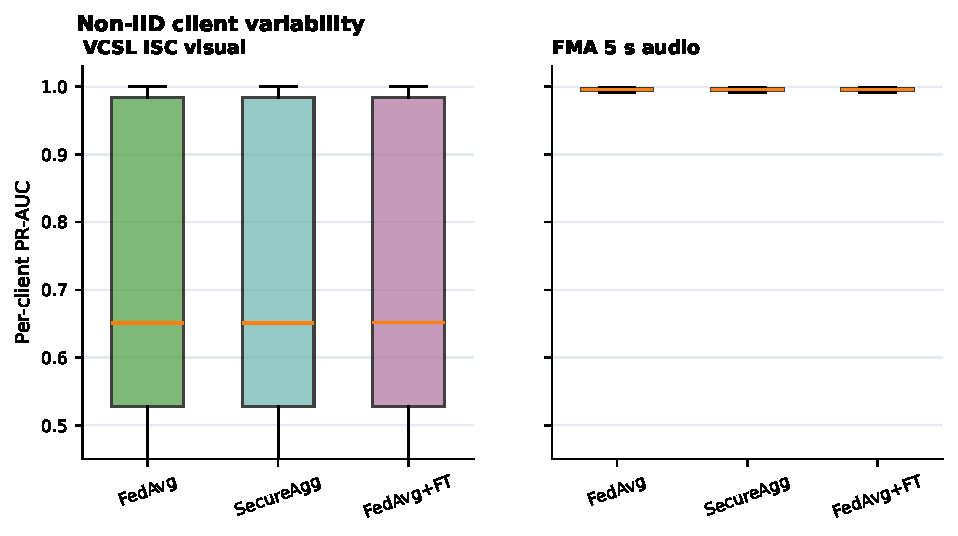
\includegraphics[width=\linewidth]{figures/fig04_client_variability.pdf}
  \end{minipage}\hfill
  \begin{minipage}{0.32\textwidth}
    \centering
    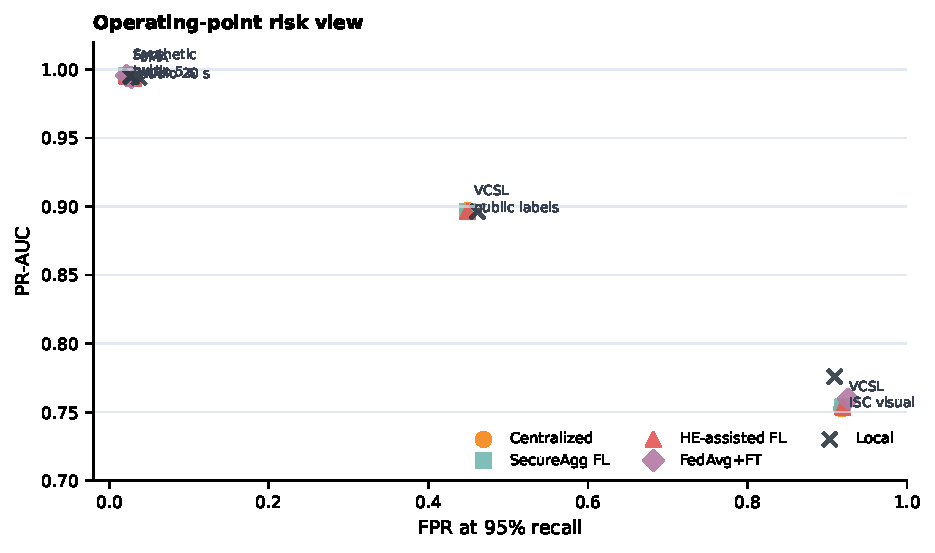
\includegraphics[width=\linewidth]{figures/fig05_operating_point_risk.pdf}
  \end{minipage}
  \caption{Supporting result views. Left: gain from the best single branch to the fused privacy-preserving model. Middle: non-IID client variability in released VCSL ISC visual descriptors and FMA short clips. Right: PR-AUC must be interpreted with FPR@95R because high-recall visual operating points remain risky.}
  \label{fig:supporting-results}
\end{figure*}

\subsection{Fixed-Evidence Audit and Feature Policy}

\begin{table*}[!t]
\centering
\caption{Exploratory archived VCSL public-label ablation. Score-only calibration is slightly strongest, while the default invariant policy remains competitive and avoids direct client/category context fields.}
\label{tab:audit-ablation}
\scriptsize
\begin{tabularx}{\textwidth}{p{0.28\textwidth} r r p{0.28\textwidth} r}
\toprule
Audit baseline & PR-AUC & FPR@95R & Feature policy & PR-AUC \\
\midrule
Logistic score-only & \textbf{0.9001}$\pm$0.0132 & 0.4452 & Score only & \textbf{0.9001}$\pm$0.0132 \\
Logistic poly2 invariant & 0.8989$\pm$0.0128 & 0.4459 & Default invariant & 0.8989$\pm$0.0128 \\
FedYogi & 0.8931$\pm$0.0117 & 0.4551 & Visual+temporal & 0.8822$\pm$0.0172 \\
FedAdam & 0.8924$\pm$0.0109 & 0.4556 & Remove reliability & 0.8405$\pm$0.0127 \\
Mean-score fusion & 0.8854$\pm$0.0124 & 0.4744 & All fields minus context & 0.8631$\pm$0.0116 \\
Hist. gradient boosting & 0.8852$\pm$0.0135 & 0.4904 & All fields & 0.8326$\pm$0.0105 \\
Video similarity & 0.8780$\pm$0.0173 & 0.5165 & Audio only & 0.8138$\pm$0.0070 \\
\bottomrule
\end{tabularx}
\end{table*}

Table~\ref{tab:audit-ablation} gives an exploratory isolation of the calibration layer under fixed pair evidence. Score-only logistic calibration is slightly strongest on this archived subset, while the invariant head is competitive. The score-only 20-D map uses video score, audio score, temporal score, maximum modality score, and mean modality score plus their squares and pairwise products. The default invariant map replaces direct context with reliability-weighted and modality-product terms. Using all fields performs worse and creates severe context leakage, which motivates excluding direct client/category fields from the default detector, but a fresh checksum-verified rerun is required before treating this ablation as confirmatory. The empirical claim is therefore deliberately modest: \ours{} provides leakage-aware federated calibration and signed audit logging over fixed evidence, not superior pair-evidence fusion on every subset and not a new descriptor or retrieval method.

\begin{figure*}[!t]
  \centering
  \begin{minipage}{0.48\textwidth}
    \centering
    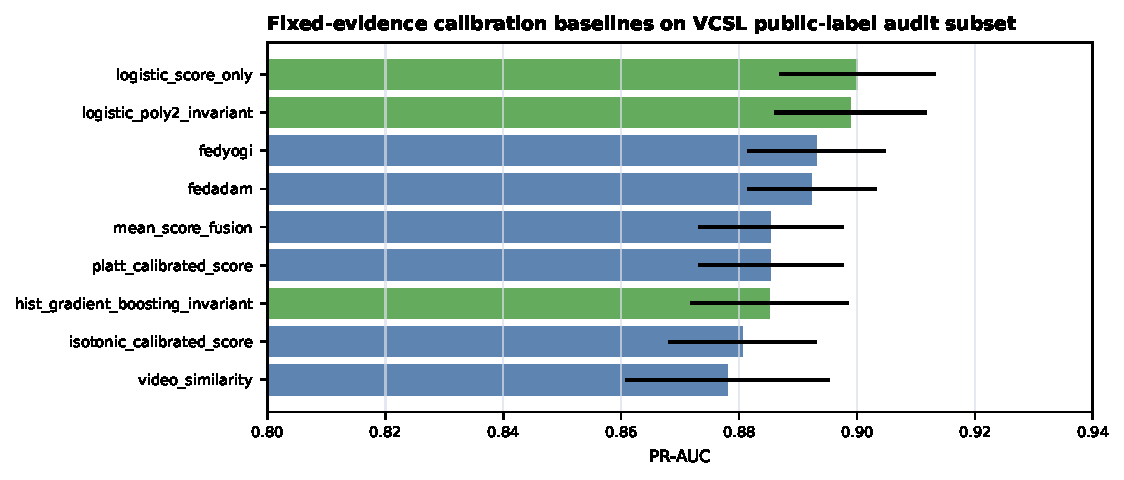
\includegraphics[width=\linewidth]{figures/fig09_fixed_evidence_baselines.pdf}
  \end{minipage}\hfill
  \begin{minipage}{0.48\textwidth}
    \centering
    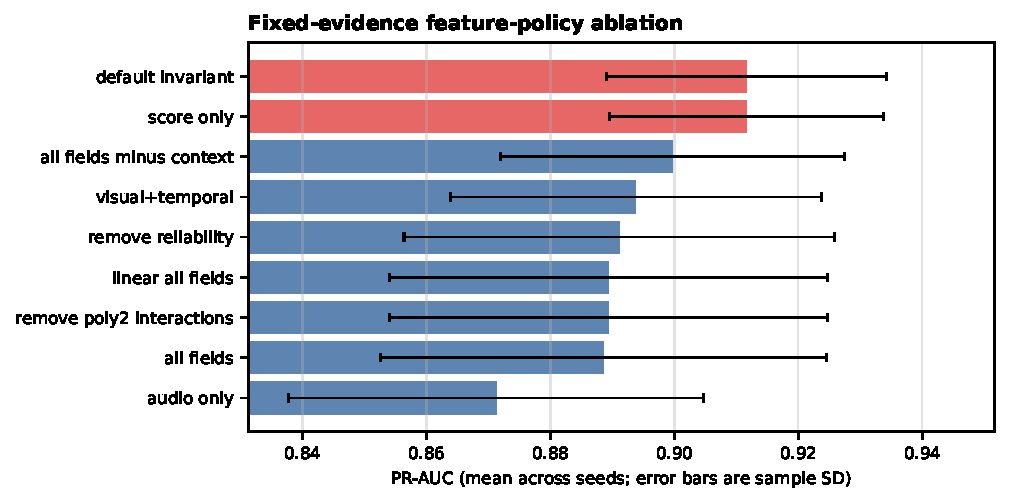
\includegraphics[width=\linewidth]{figures/fig10_feature_ablation.pdf}
  \end{minipage}
  \caption{Exploratory archived audit-subset evidence. Left: fixed-evidence calibration baselines. Right: feature ablation motivating exclusion of direct context fields from the default detector; a fresh input-verifiable rerun is required for a confirmatory claim.}
  \label{fig:audit-ablation}
\end{figure*}

\subsection{Query Ranking, Open-Set Stress, and Prevalence Risk}

\begin{table*}[!t]
\centering
\caption{Three-seed mean query-ranking metrics on asset-disjoint VCSL public-label candidate pools. The 1:10000 row is a candidate-instance stress with repeated references/noise realizations, not 10,000 unique references per query.}
\label{tab:query-ranking}
\scriptsize
\begin{tabularx}{\textwidth}{p{0.19\textwidth} r r r r r r}
\toprule
Method / ratio & Queries & Pairs & R@1 & R@10 & R@100 & mAP \\
\midrule
Score-only, 1:1 & 540 & 1,800 & 0.9528 & 1.0000 & 1.0000 & 0.9607 \\
Invariant, 1:1 & 540 & 1,800 & 0.9536 & 1.0000 & 1.0000 & 0.9613 \\
Score-only, 1:100 & 192 & 22,220 & 0.3462 & 0.7547 & 1.0000 & 0.4639 \\
Invariant, 1:100 & 192 & 22,220 & 0.3284 & 0.7683 & 1.0000 & 0.4547 \\
Score-only, 1:1000 & 100 & 100,100 & 0.1633 & 0.3967 & 0.7900 & 0.2468 \\
Invariant, 1:1000 & 100 & 100,100 & 0.1400 & 0.3933 & 0.7933 & 0.2253 \\
Score-only, 1:10000 & 100 & 1,000,100 & 0.0567 & 0.1800 & 0.4067 & 0.1019 \\
Invariant, 1:10000 & 100 & 1,000,100 & 0.0600 & 0.1867 & 0.3900 & 0.0985 \\
\bottomrule
\end{tabularx}
\end{table*}

\begin{figure*}[!t]
  \centering
  \begin{minipage}{0.48\textwidth}
    \centering
    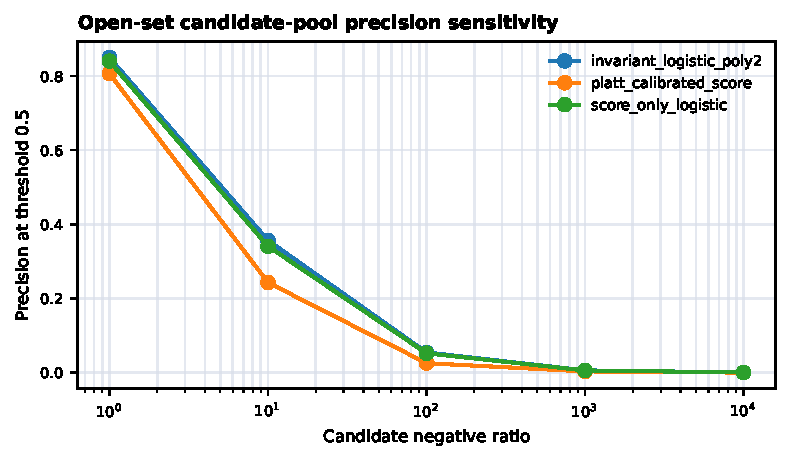
\includegraphics[width=\linewidth]{figures/open_set_precision_curves.pdf}
  \end{minipage}\hfill
  \begin{minipage}{0.48\textwidth}
    \centering
    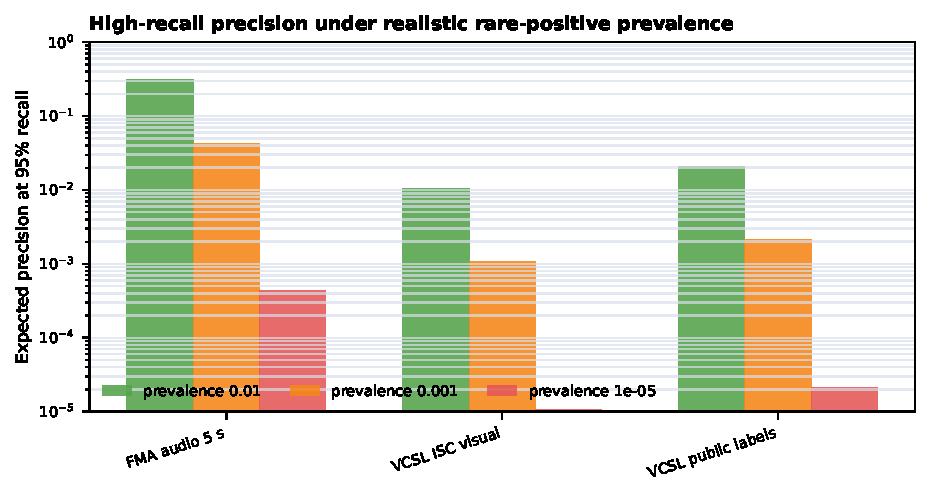
\includegraphics[width=\linewidth]{figures/fig12_prevalence_precision.pdf}
  \end{minipage}
  \caption{Deployment-risk view. Left: precision at threshold 0.5 drops as candidate negative ratio increases. Right: expected high-recall precision under rare-positive prevalence, derived from measured FPR@95R and a 95\% recall target.}
  \label{fig:deployment-risk}
\end{figure*}

\begin{table*}[!t]
\centering
\caption{Representative operating-point metrics on held-out pairs. Precision and recall use threshold $0.5$; FPR@95R is obtained by threshold sweep.}
\label{tab:operating-metrics}
\scriptsize
\begin{tabularx}{\textwidth}{p{0.17\textwidth} p{0.23\textwidth} r r r}
\toprule
Tier & Method & Precision & Recall & FPR@95R \\
\midrule
VCSL public labels & Centralized fused & 0.8496 & 0.8196 & 0.3696 \\
VCSL public labels & SecureAgg FedAvg & 0.8553 & 0.8063 & 0.3693 \\
VCSL public labels & Local multimodal & 0.8586 & 0.8048 & 0.3681 \\
VCSL ISC visual & Video similarity & 0.9393 & 0.4424 & 0.9138 \\
VCSL ISC visual & Personalized FedAvg & 0.9460 & 0.4409 & 0.9262 \\
VCSL ISC visual & Local multimodal & 0.9568 & 0.4216 & 0.9093 \\
FMA audio 5 s & Audio similarity & 0.5169 & 1.0000 & 0.1487 \\
FMA audio 5 s & SecureAgg FedAvg & 0.9219 & 0.9894 & 0.0224 \\
FMA audio 5 s & Personalized FedAvg & 0.9239 & 0.9894 & 0.0214 \\
\bottomrule
\end{tabularx}
\end{table*}

Table~\ref{tab:query-ranking}, Table~\ref{tab:operating-metrics}, and Fig.~\ref{fig:deployment-risk} expose retrieval-like behavior that pair PR-AUC alone hides. Score-only remains slightly stronger than the invariant head in most public-label ranking slices, and both degrade under 1:100, 1:1000, and 1:10000 candidate-instance pools. Every hardest-ratio seed contains 100 positive-bearing queries and 1,000,100 candidate instances; because the public label topology contains fewer than 10,001 unique references, repeated reference assets and noise realizations are used and the result is not a unique-reference retrieval benchmark. At 1\% prevalence and 95\% recall, expected precision is only about 2.5\% for the asset-disjoint VCSL public-label SecureAgg result. These false-positive rates are inappropriate for automated enforcement. The appropriate deployment role is candidate prioritization followed by human review, ownership validation, and appeal or supersession procedures.

\subsection{Additional Stress Tests}

\begin{figure*}[!t]
  \centering
  \begin{minipage}{0.32\textwidth}
    \centering
    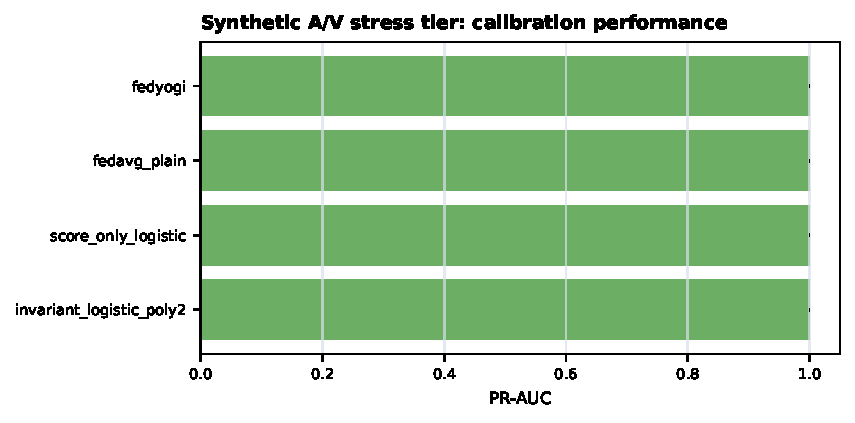
\includegraphics[width=\linewidth]{figures/av_sync_tier_pr_auc.pdf}
  \end{minipage}\hfill
  \begin{minipage}{0.32\textwidth}
    \centering
    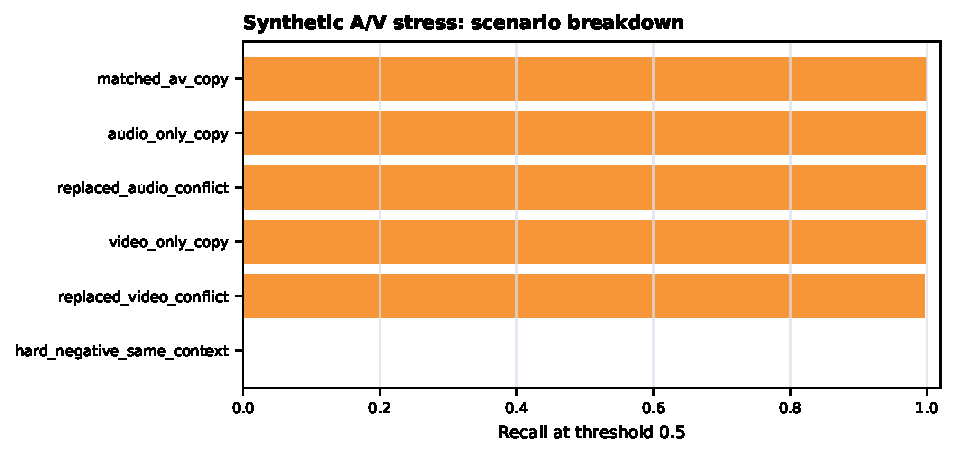
\includegraphics[width=\linewidth]{figures/av_conflict_breakdown.pdf}
  \end{minipage}\hfill
  \begin{minipage}{0.32\textwidth}
    \centering
    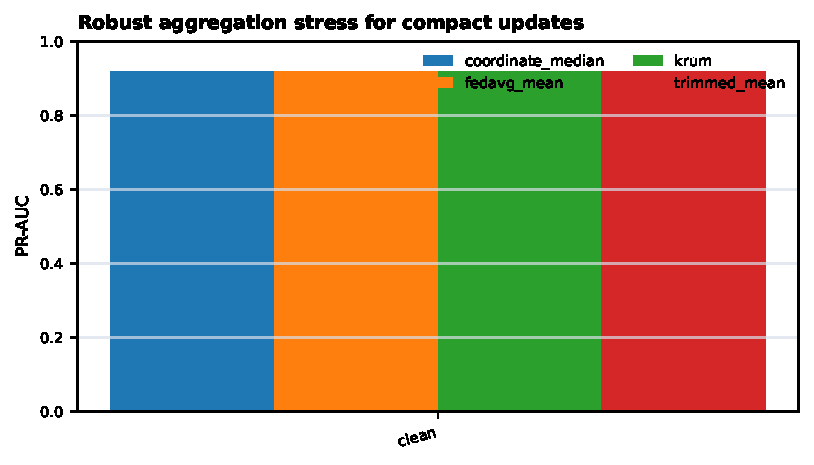
\includegraphics[width=\linewidth]{figures/robust_aggregation_stress.pdf}
  \end{minipage}
  \caption{Stress-test diagnostics. Left/middle: synthetic A/V conflict tier, which is not natural synchronized audiovisual evidence. Right: 20-round compact-head stress across label-flip/sign-flip attacks and 0\%, 10\%, and 20\% attacker fractions; this is not a Byzantine-security proof.}
  \label{fig:stress-tests}
\end{figure*}

A synthetic A/V conflict tier tests modality disagreement because a natural synchronized public audio-video piracy corpus is not included in this artifact. FedAdam and FedYogi reach 0.99997 PR-AUC, FedAvg reaches 0.99986, invariant logistic reaches 0.99982, and naive mean-score fusion drops to 0.93613 with FPR@95R 0.8886. The tier is an engineering stress test, not natural A/V evidence. The poisoning audit runs 20 communication rounds for seeds 31, 37, and 41 with 0\%, 10\%, and 20\% attackers under label-flip and sign-flip perturbations. Mean, coordinate-median, trimmed-mean, and Krum aggregation are compared on the same frozen test rows. This remains a controlled compact-head diagnostic rather than a Byzantine-security guarantee; aggregate utility and attack-induced degradation are reported in the released table.

\subsection{Protected Aggregation, Leakage, and Receipts}

\begin{figure*}[!t]
  \centering
  \begin{minipage}{0.48\textwidth}
    \centering
    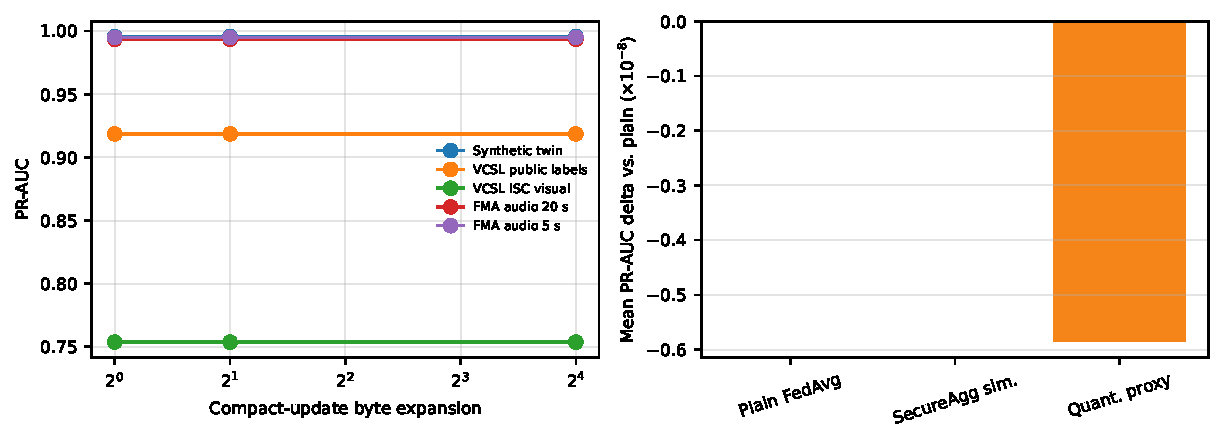
\includegraphics[width=\linewidth]{figures/fig03_privacy_utility_tradeoff.pdf}
  \end{minipage}\hfill
  \begin{minipage}{0.48\textwidth}
    \centering
    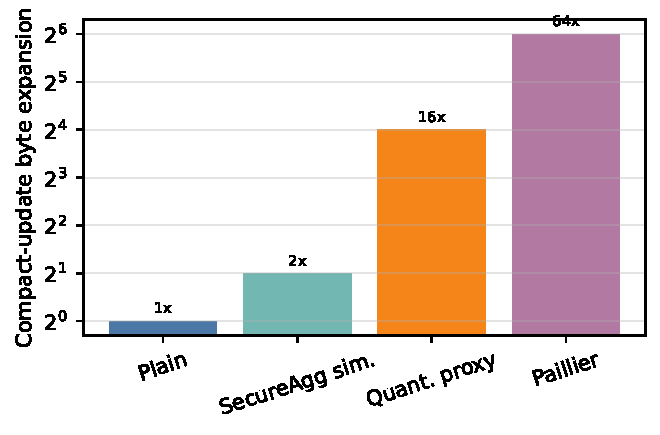
\includegraphics[width=\linewidth]{figures/fig06_crypto_overhead.pdf}
  \end{minipage}
  \caption{Protected-update accounting. Left: SecureAgg simulation and the quantized transport proxy preserve compact-head FedAvg utility within numerical tolerance. Right: compact-head communication expansion must not be extrapolated to ciphertext-domain media scoring.}
  \label{fig:protected-overhead}
\end{figure*}

\begin{table*}[!t]
\centering
\caption{Privacy, receipt, and protected-aggregation diagnostics. These diagnostics support raw-media non-export and auditability, not formal privacy or production cryptography.}
\label{tab:diagnostics}
\scriptsize
\begin{tabularx}{\textwidth}{p{0.23\textwidth} p{0.23\textwidth} p{0.18\textwidth} X}
\toprule
Diagnostic & Setting & Result & Interpretation \\
\midrule
Client identity leakage & All fields vs. invariant & 1.0000 vs. 0.1115$\pm$0.0207 & Direct context fields leak client identity; invariant policy is near 11-client chance. \\
Query category leakage & All fields vs. invariant & 1.0000 vs. 0.1020$\pm$0.0130 & Category/context fields should not be default detector inputs. \\
Membership attack & Best tested scalar/model attack & AUC 0.5780$\pm$0.0170 & Weak but nonzero signal; no differential-privacy guarantee is claimed. \\
Receipt verification & 1000 receipts/seed & 100\% verify and tamper detect & Signed salted hash chains support commitment audit without storing media. \\
Paillier compact sum & 8 clients, 24-D updates, 2048-bit key & $64\times$ bytes, $2.64\times10^{-7}$ max error & Real additive sum; 21.68 s encryption and 2.07 s aggregate/decrypt in this local microbenchmark. \\
SecureAgg/proxy status & Pairwise-mask simulation / quantized proxy & $\leq2.86\times10^{-15}$ dropout error & Arithmetic recovery holds at 0\%, 10\%, and 20\% dropout; neither mode is production cryptography. \\
\bottomrule
\end{tabularx}
\end{table*}

The protected-update audit separates three mechanisms. SecureAgg simulation tests pairwise-mask cancellation with 0\%, 10\%, and 20\% client dropout; the quantized transport proxy reports numeric and byte effects without claiming encryption; real Paillier encrypts quantized compact updates, sums ciphertexts additively, decrypts only the aggregate, and compares the result with the plain weighted update. Table~\ref{tab:diagnostics} summarizes the privacy and audit diagnostics: context fields can leak identity, membership attacks are weak but nonzero, receipts verify deterministically, and protected aggregation is not a substitute for differential privacy, production dropout recovery, threshold keys, or full encrypted inference.

\begin{figure*}[!t]
  \centering
  \begin{minipage}{0.48\textwidth}
    \centering
    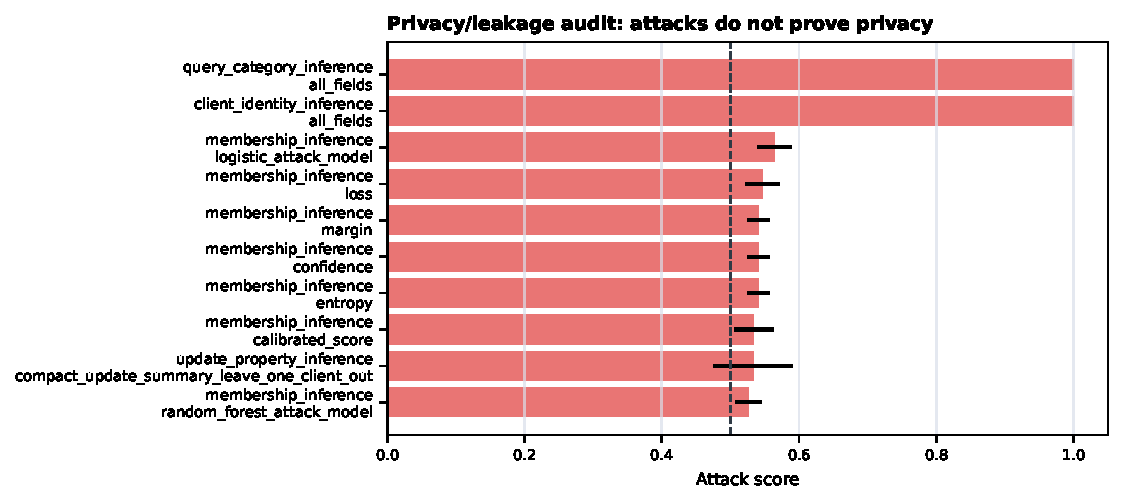
\includegraphics[width=\linewidth]{figures/privacy_attack_summary.pdf}
  \end{minipage}\hfill
  \begin{minipage}{0.48\textwidth}
    \centering
    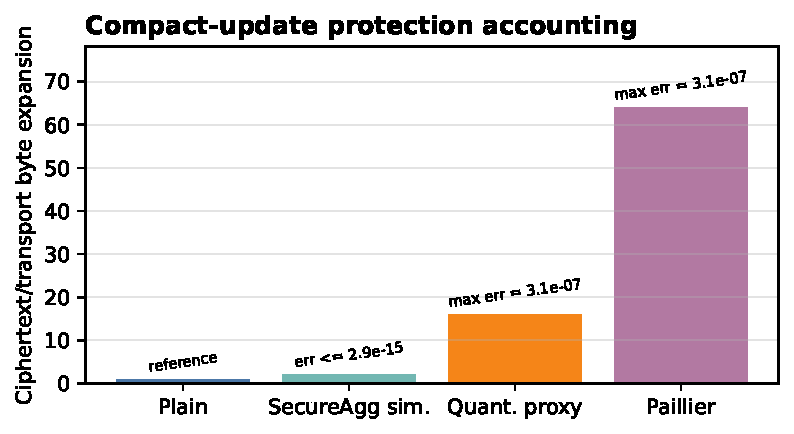
\includegraphics[width=\linewidth]{figures/paillier_update_overhead.pdf}
  \end{minipage}
  \caption{Additional privacy and cryptographic accounting. Left: expanded privacy/leakage audit; values above chance indicate leakage signals but do not prove privacy failure alone. Right: byte expansion for plain, quantized-proxy, and real Paillier compact-head update aggregation.}
  \label{fig:privacy-paillier}
\end{figure*}

\section{Discussion}

The results support the main claim that a compact fixed-evidence calibration and audit layer can be trained across clients while preserving compact-head utility under protected-update accounting. They also show that signed evidence anchoring can be added without storing media or embeddings in the ledger. The query-ranking and prevalence analyses make the deployment boundary clearer: calibrated scores can prioritize candidate review, but performance degrades as hard negatives increase, especially in the 1:10000 candidate-instance stress. The exploratory feature ablation and the checksum-verified leakage audit both motivate excluding direct client/category fields from default detector inputs. The Paillier experiment shows real additive encrypted summation is feasible for compact updates, with substantial byte and runtime costs.

The results do not prove that \ours{} solves piracy detection in the wild. VCSL validates the visual branch and FMA validates the audio branch, but the paper does not yet include a natural synchronized audio-video piracy corpus. The evaluation also does not establish superiority over ViSiL/FIVR-style retrieval and localization systems because those systems are treated as upstream evidence providers rather than replaced baselines. The protected aggregation mechanisms keep raw media local and model aggregate-only update visibility under an honest-but-curious setting; they do not provide differential privacy, collusion resistance, malicious-client robustness proof, or protection against all update-leakage attacks. The receipt ledger supports auditability; it does not prevent piracy, establish ownership, certify feature-extraction correctness, or replace human review.

For multimedia systems, the intended role is a layer between specialized visual retrieval/audio fingerprinting engines and rights-management or human-review workflows. Upstream engines generate candidate evidence, \ours{} trains and calibrates the compact head across clients, and the receipt protocol records media-free audit commitments. Ethical deployment requires human review, appeal channels, ownership verification, and documented supersession of mistaken receipts before any enforcement action.

\section{Reproducibility and Ethics}

The public implementation package contains benchmark runners, feature construction, compact-head training, protected-aggregation simulation, Paillier compact-update aggregation, signed receipt chains, canonical test vectors, permitted CSV/JSON evidence, configuration files, run manifests, table/figure sources, and SHA-256 checksums at \url{https://github.com/Devchandrasen/fedtwin-cryptid}. The release excludes copyrighted media, downloaded descriptors, caches, bytecode, temporary files, and private paths. A frozen archival DOI will be inserted only after the verified GitHub release is deposited; no placeholder DOI is used.

Ethically, the system should be used as review triage, not automatic takedown authority. High false-positive rates at high recall can create wrongful enforcement risk, especially at realistic low prevalence. A dominant platform or rights holder could misuse calibrated scores or receipts against smaller creators, so contested claims require transparent disclosure, independent review, and a path to retract or supersede mistaken decisions. The receipt chain records commitments and ordering; it does not prove infringement, ownership, intent, or legal liability. The media-free design reduces raw-media exposure but does not remove all privacy risk because model updates and scores can leak statistical information.

\subsection{Limitations and Next Validation}

The current evaluation deliberately separates what the system demonstrates from what remains unresolved. First, VCSL validates visual evidence and FMA validates audio evidence, but a natural synchronized A/V piracy corpus is not included. The synthetic A/V conflict tier is useful for testing modality disagreement, yet future work needs a rights-cleared synchronized benchmark with transformations that affect one or both modalities. Second, the query-ranking metrics use public label/topology candidate pools and do not replace segment-overlap localization metrics. The next validation should run the calibration layer on top of ViSiL/FIVR/VCSL-style segment proposals and report localization-aware precision and recall.

Third, privacy is bounded rather than formal. The artifact keeps raw media and raw embeddings local and shows that direct context fields leak identity, but it does not provide differential privacy, collusion resistance, or a complete update-leakage defense. Fourth, the 20-round poisoning matrix remains a controlled compact-head stress, not a proof against adaptive Byzantine clients. Finally, cryptography is compact-update only: SecureAgg is simulated, quantization is a transport proxy, and Paillier sums compact updates. Production use would require authenticated dropout recovery, threshold keys, key lifecycle management, and possibly encrypted inference for selected compact features.

\section{Conclusion}

This paper presented \ours, a federated fixed-evidence calibration and audit layer for multimedia copy review. The method integrates media-free pair states, compact-head federated calibration, protected-update accounting, personalization analysis, leakage-aware feature policy, Paillier compact-update summation, query-ranking diagnostics, and signed receipt chains. Across VCSL and FMA tiers, protected federated variants preserve compact-head utility, but open-set and prevalence analyses show that the system should be used for review triage rather than automated enforcement. Future work should add synchronized public audio-video copy-review corpora, stronger VCDB/FIVR/VCSL localization validation, formal privacy accounting, malicious-client robustness, and production cryptographic protocols.

\bibliographystyle{IEEEtran}
\bibliography{references}

\end{document}
